\documentclass{article}
\usepackage{graphicx}
\usepackage{booktabs}
\usepackage[margin=1in]{geometry}

\usepackage{float}  % <-- Added to fix [H] errors
\usepackage{adjustbox}  % <-- Allows resizing wide tables

\begin{document}

\title{Generated Model Performance Report}
\author{Simon Green}
\date{\today}
\maketitle

\section*{Results and Model Comparison} 

This report presents the performance evaluation of six reinforcement learning models: EnTRPO, GenTRPO, TRPO, PPO, and TRPOR. The comparison is based on reward statistics across different environments. We present the data but do not draw any conclusions from it in this report.

\subsection*{Model Performance Table}

The table below summarizes the performance of different models in terms of mean and standard deviation of rewards, along with maximum and minimum rewards recorded during training. A higher mean reward indicates better average performance, while a lower standard deviation suggests more stability.

\bigskip

\begin{center}
  \begin{tabular}{|l|p{3.2cm}|p{3.2cm}|p{3.2cm}|p{3.2cm}|}
\toprule
 & Ant-v5 & Pendulum-v1 & InvertedDouble Pendulum-v5 & Humanoid-v5 \\
\midrule
PPO & $\begin{array}{c} 1173.61M \\ 515.51\mu \pm 326.48\sigma \\ 1895E, 10R \end{array}$ & $\begin{array}{c} -0.02M \\ -207.56\mu \pm 118.01\sigma \\ 2892E, 10R \end{array}$ & $\begin{array}{c} 9359.93M \\ 1090.87\mu \pm 2910.66\sigma \\ 6965E, 10R \end{array}$ & $\begin{array}{c} 1245.44M \\ 464.88\mu \pm 298.07\sigma \\ 15385E, 9R \end{array}$ \\  \hline
TRPO & $\begin{array}{c} 1960.61M \\ 1328.68\mu \pm 284.88\sigma \\ 1067E, 10R \end{array}$ & $\begin{array}{c} -0.20M \\ -141.97\mu \pm 115.55\sigma \\ 2600E, 10R \end{array}$ & $\begin{array}{c} 9359.78M \\ 7516.76\mu \pm 3879.62\sigma \\ 5767E, 10R \end{array}$ & $\begin{array}{c} 1247.77M \\ 369.87\mu \pm 311.76\sigma \\ 9569E, 10R \end{array}$ \\  \hline
TRPOER & $\begin{array}{c} 1349.85M \\ 639.65\mu \pm 465.91\sigma \\ 1882E, 8R \end{array}$ & $\begin{array}{c} -0.07M \\ -173.49\mu \pm 156.48\sigma \\ 2859E, 10R \end{array}$ & $\begin{array}{c} 9351.73M \\ 2673.08\mu \pm 2620.77\sigma \\ 5070E, 9R \end{array}$ & $\begin{array}{c} 897.72M \\ 371.33\mu \pm 359.99\sigma \\ 2799E, 4R \end{array}$ \\  \hline
TRPOR & $\begin{array}{c} 3590.62M \\ 1662.87\mu \pm 1171.26\sigma \\ 1655E, 7R \end{array}$ & $\begin{array}{c} -0.22M \\ -197.32\mu \pm 215.34\sigma \\ 4508E, 10R \end{array}$ & $\begin{array}{c} 9357.32M \\ 8045.50\mu \pm 2918.29\sigma \\ 9123E, 5R \end{array}$ & $\begin{array}{c} 1416.67M \\ 620.72\mu \pm 381.70\sigma \\ 9225E, 10R \end{array}$ \\  \hline
\bottomrule  \hline
\end{tabular}

\end{center}
\
\bigskip

\section*{Performance Analysis Through Plots}

To gain deeper insights into the models' behavior, the following plots provide visualizations of various performance aspects.

\subsection*{Learning Stability}

\begin{figure}[H]
    \centering
    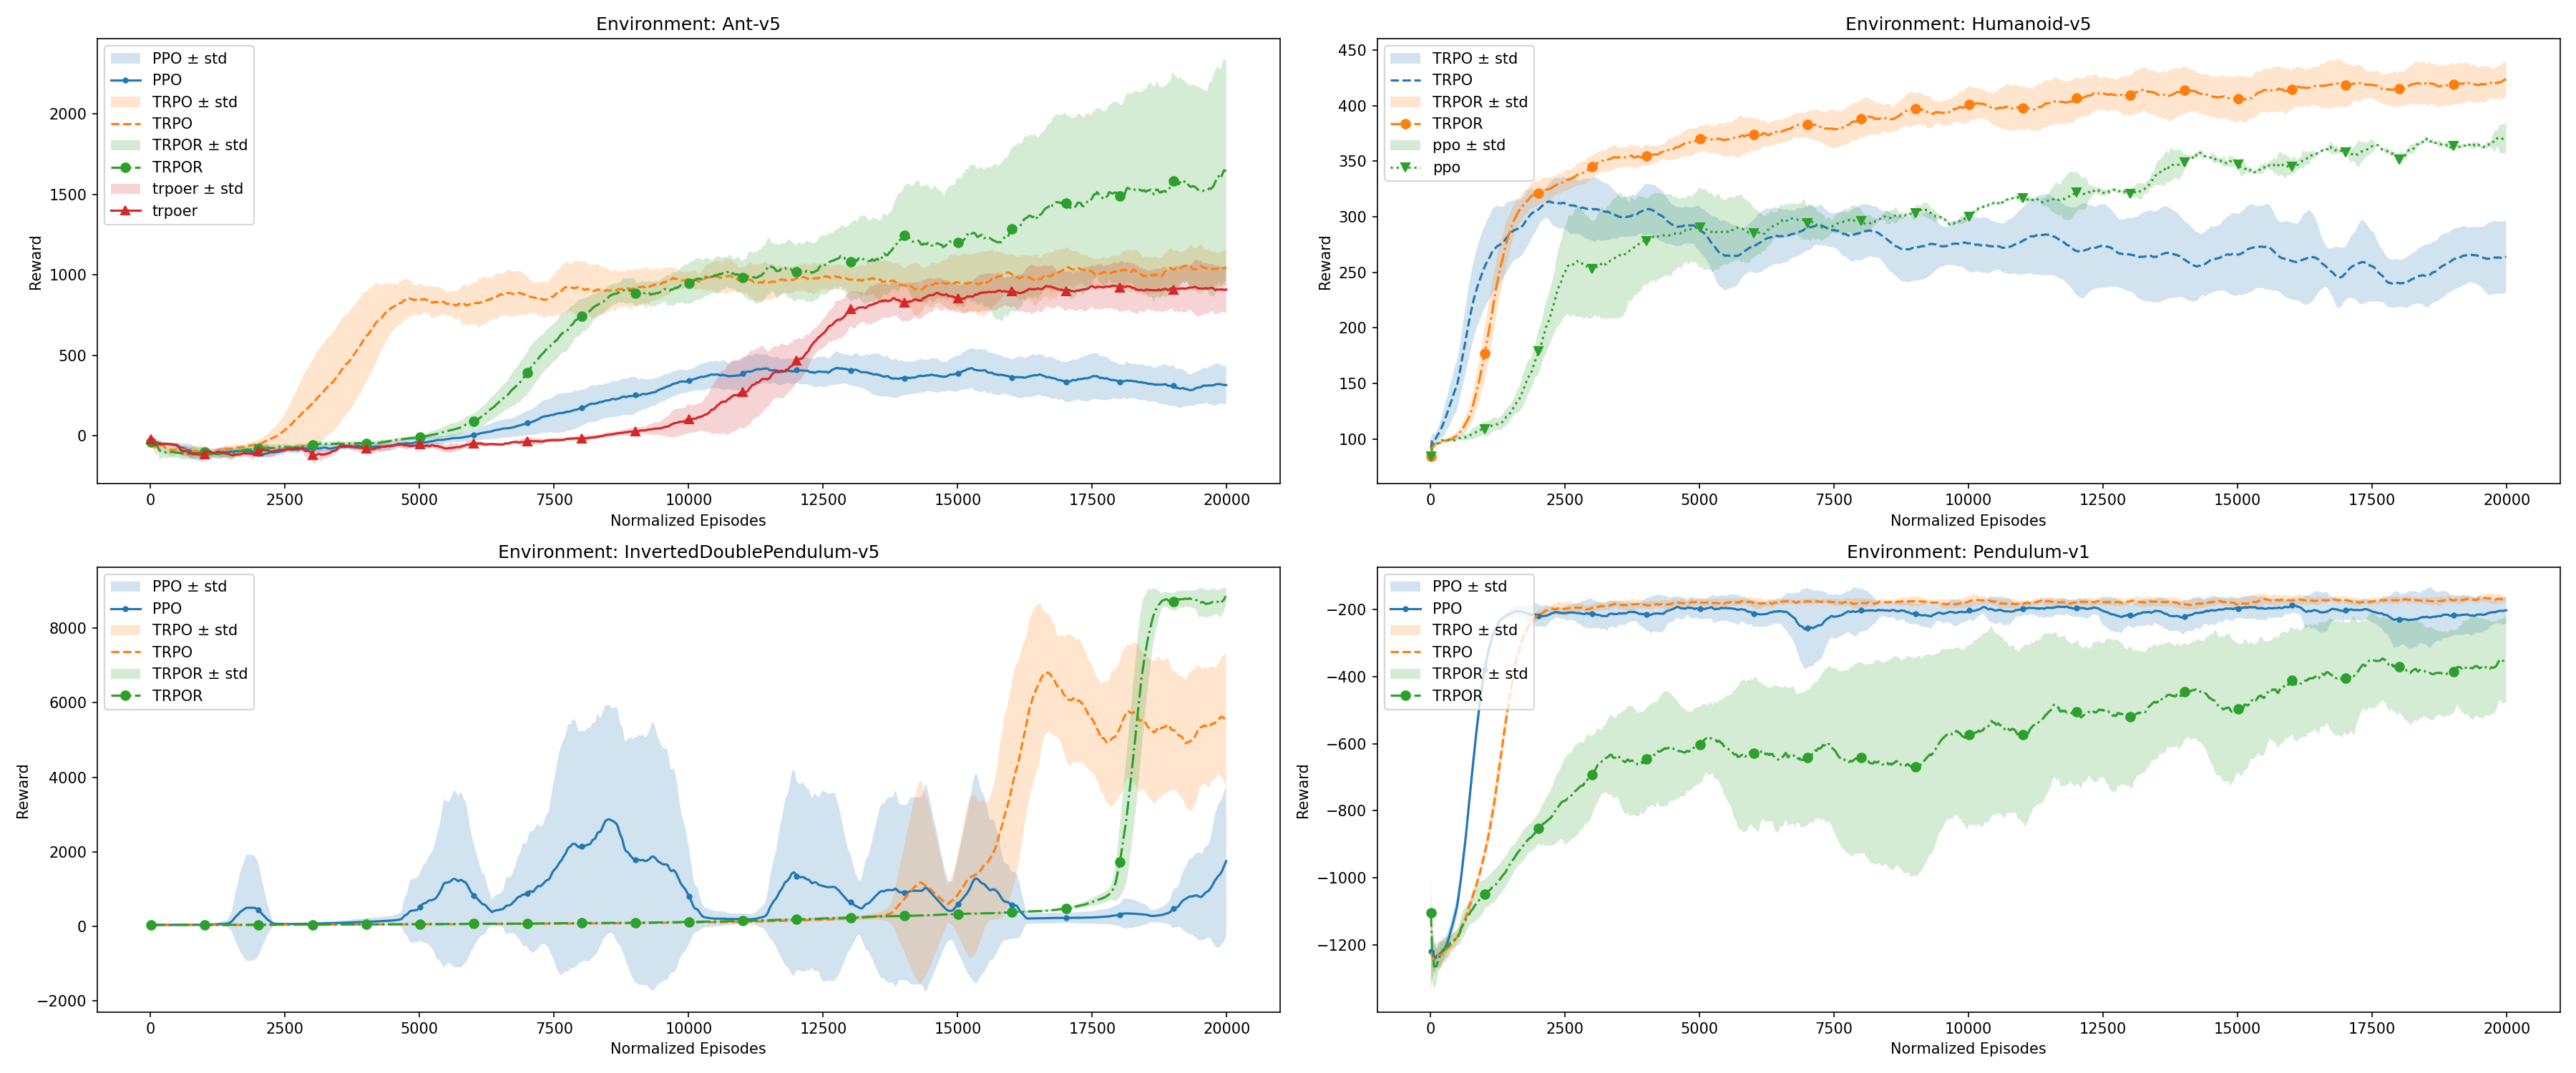
\includegraphics[width=0.8\textwidth]{.assets/learning_stability.png}
    \caption{Learning Stability for Different Models}
\end{figure}

Learning stability measures how consistent a model's performance is over time. A smoother and more steadily increasing reward curve indicates that the model is learning in a reliable and predictable manner. Models with high variance in their learning curves may be struggling with instability or sensitivity to hyperparameters.

\subsection*{Learning Stability (Coefficient of Variation)}

\begin{figure}[H]
    \centering
    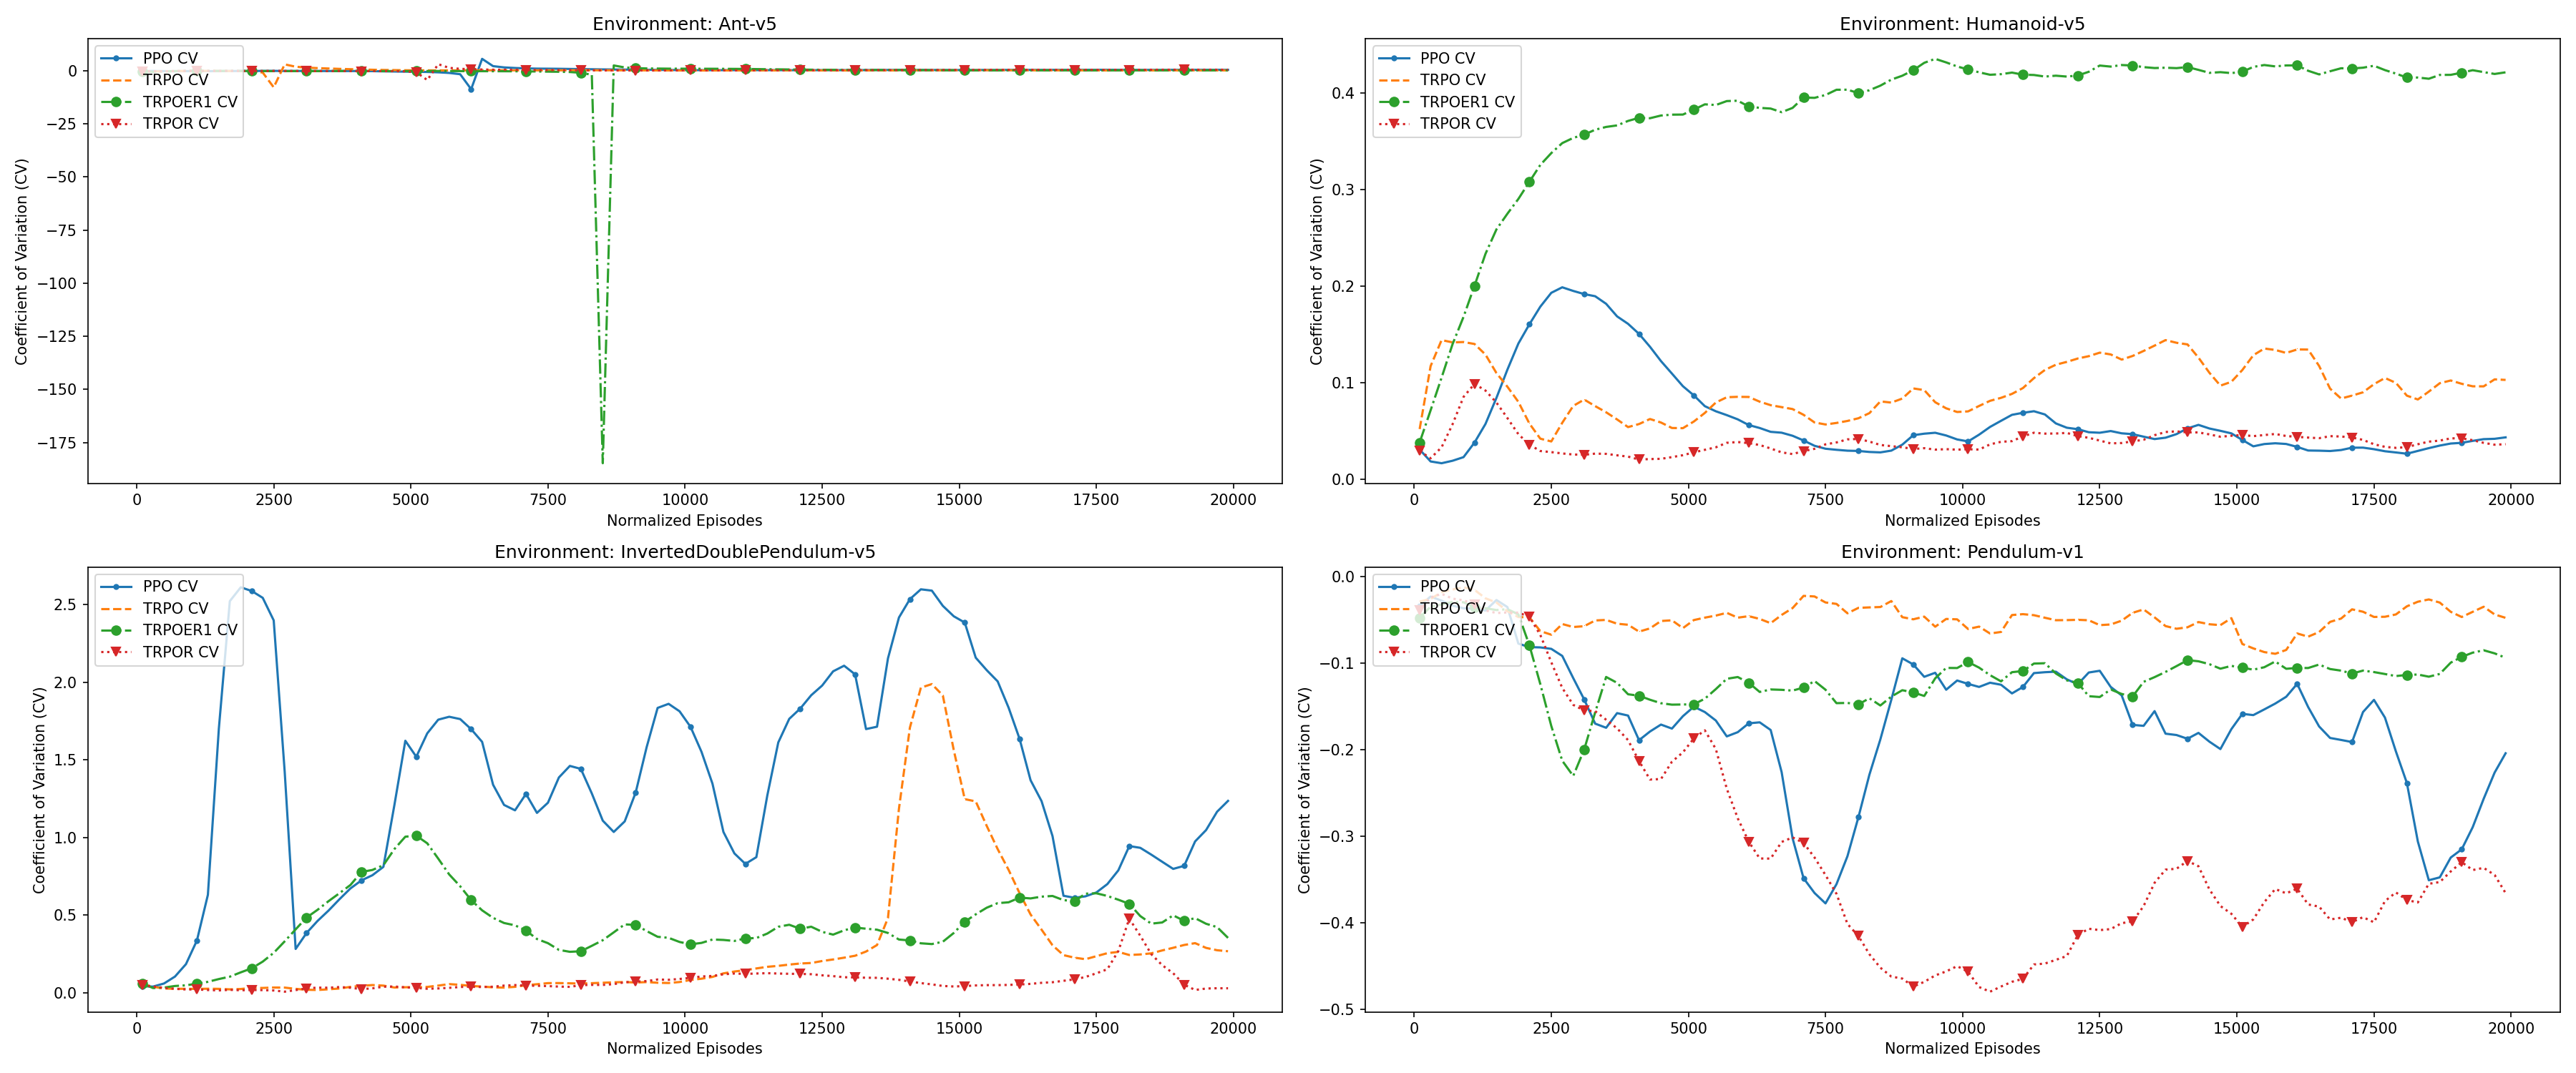
\includegraphics[width=0.8\textwidth]{.assets/learning_stability_cv.png}
    \caption{Learning Stability (Coefficient of Variation)}
\end{figure}

The coefficient of variation (CV) provides a normalized measure of learning stability. A lower CV indicates that the model's performance is less volatile, meaning it generalizes better across different training runs. High CV values suggest inconsistent learning, which could be due to stochasticity in training or sensitivity to random seeds.

\subsection*{Sample Efficiency}

\begin{figure}[H]
    \centering
    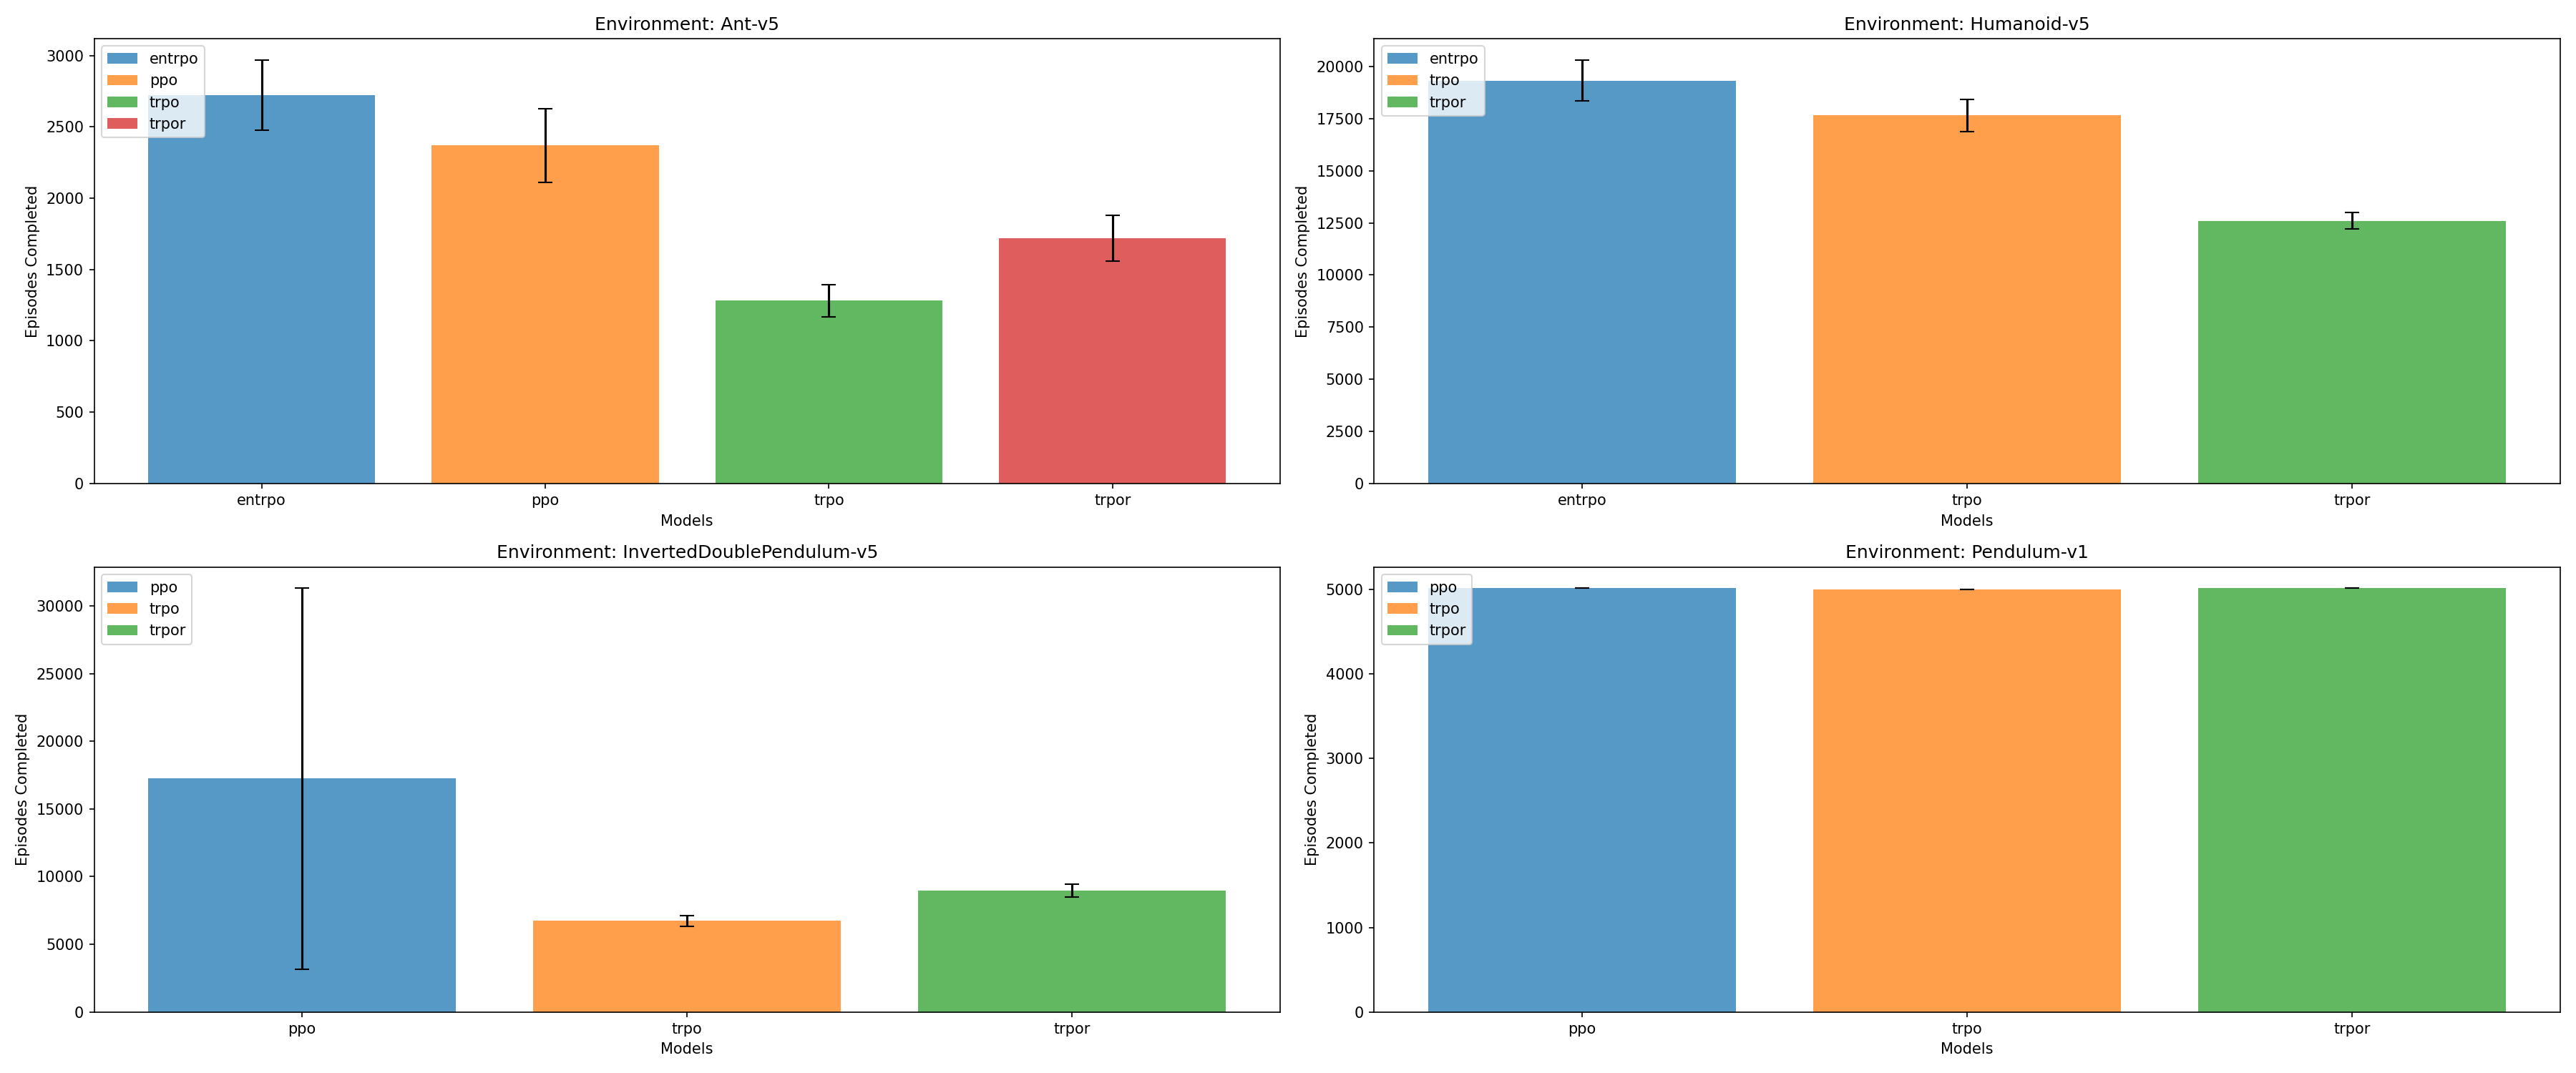
\includegraphics[width=0.8\textwidth]{.assets/sample_efficiency.png}
    \caption{Sample Efficiency Across Models}
\end{figure}

Sample efficiency refers to how quickly a model improves given a limited number of training episodes. Models that reach higher rewards with fewer episodes are considered more sample-efficient. This metric is crucial in real-world applications where data collection is expensive or time-consuming.

\subsection*{Combined Sample Efficiency Results}

\begin{figure}[H]
    \centering
    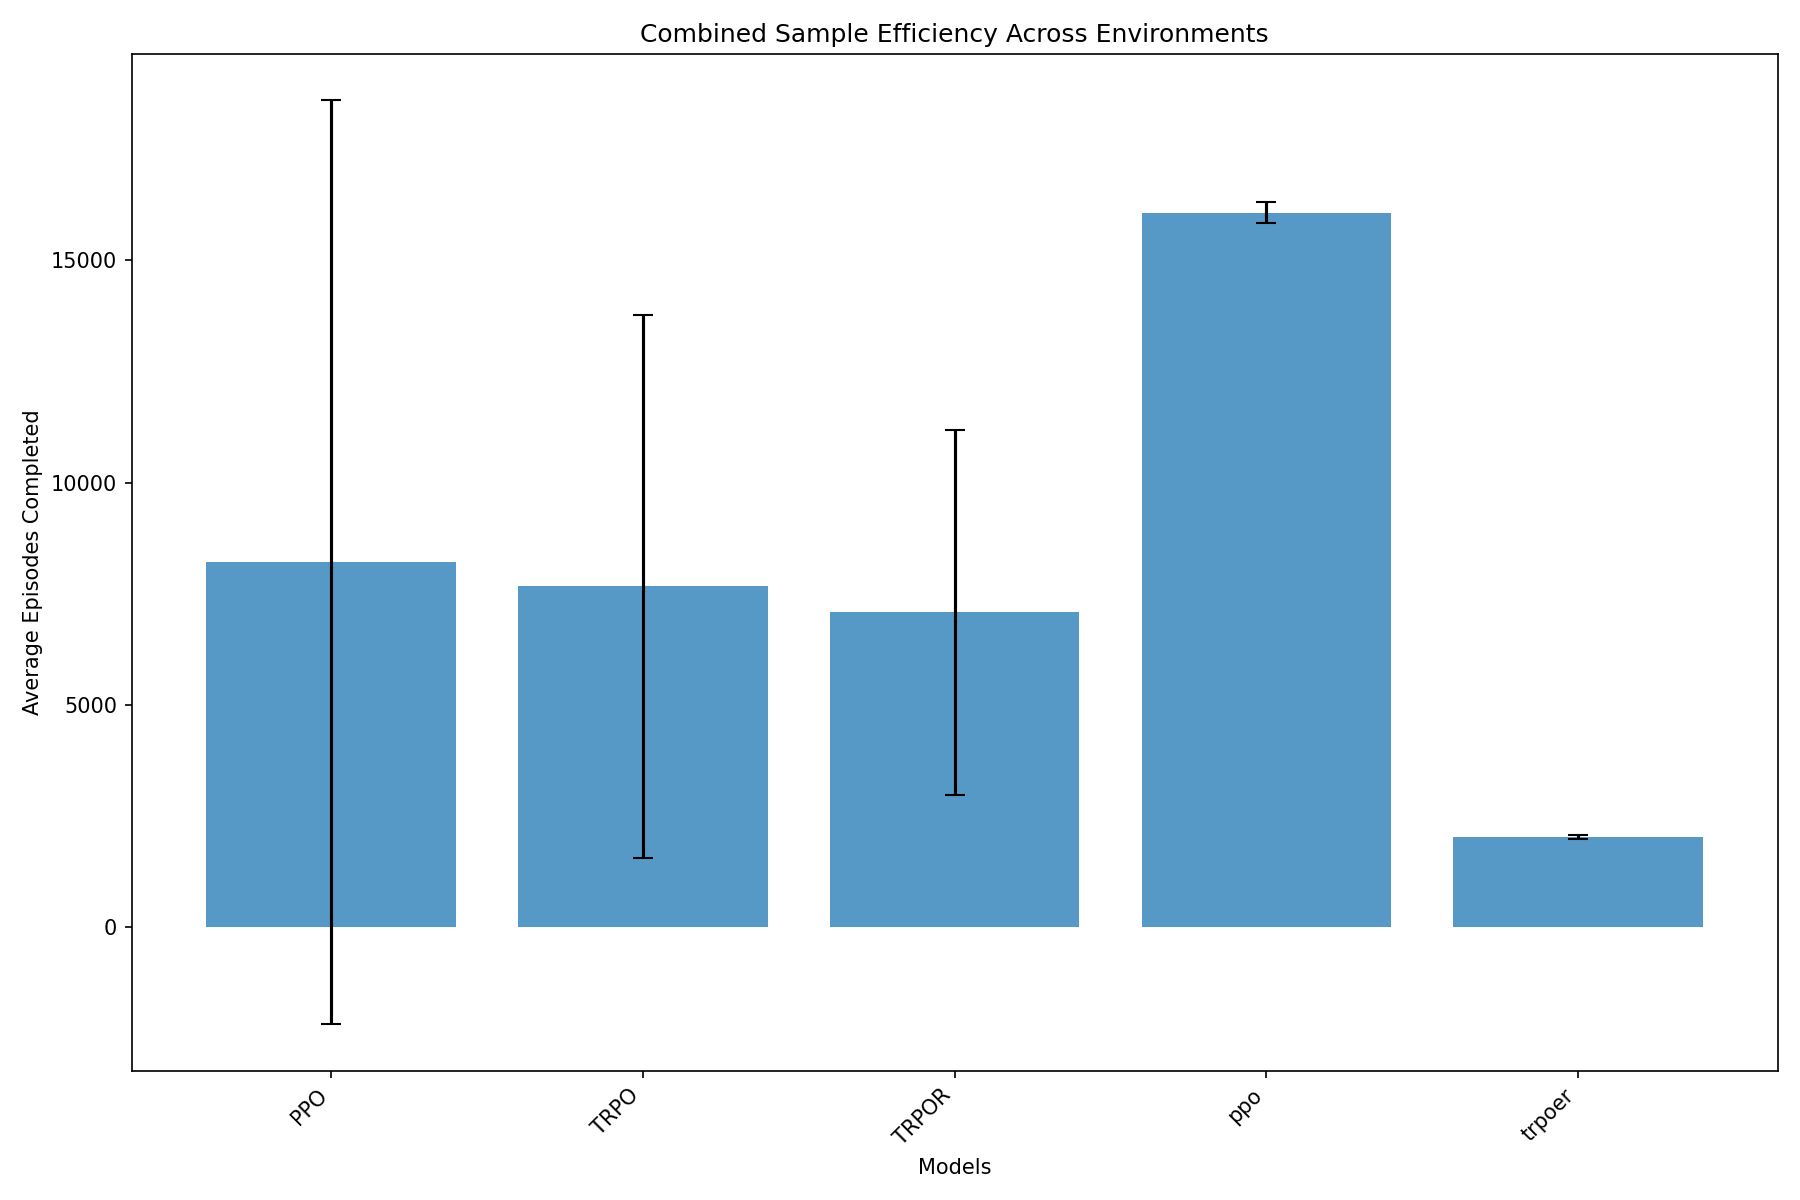
\includegraphics[width=0.8\textwidth]{.assets/sample_efficiency_combined.png}
    \caption{Combined Sample Efficiency Results}
\end{figure}

This combined sample efficiency plot compares models across all environments, showing which algorithms consistently require fewer interactions to achieve optimal performance. A model with consistently high sample efficiency is preferable for scenarios where training costs are high.

\subsection*{Resampled Rewards and Outlier Removal}

\begin{figure}[H]
    \centering
    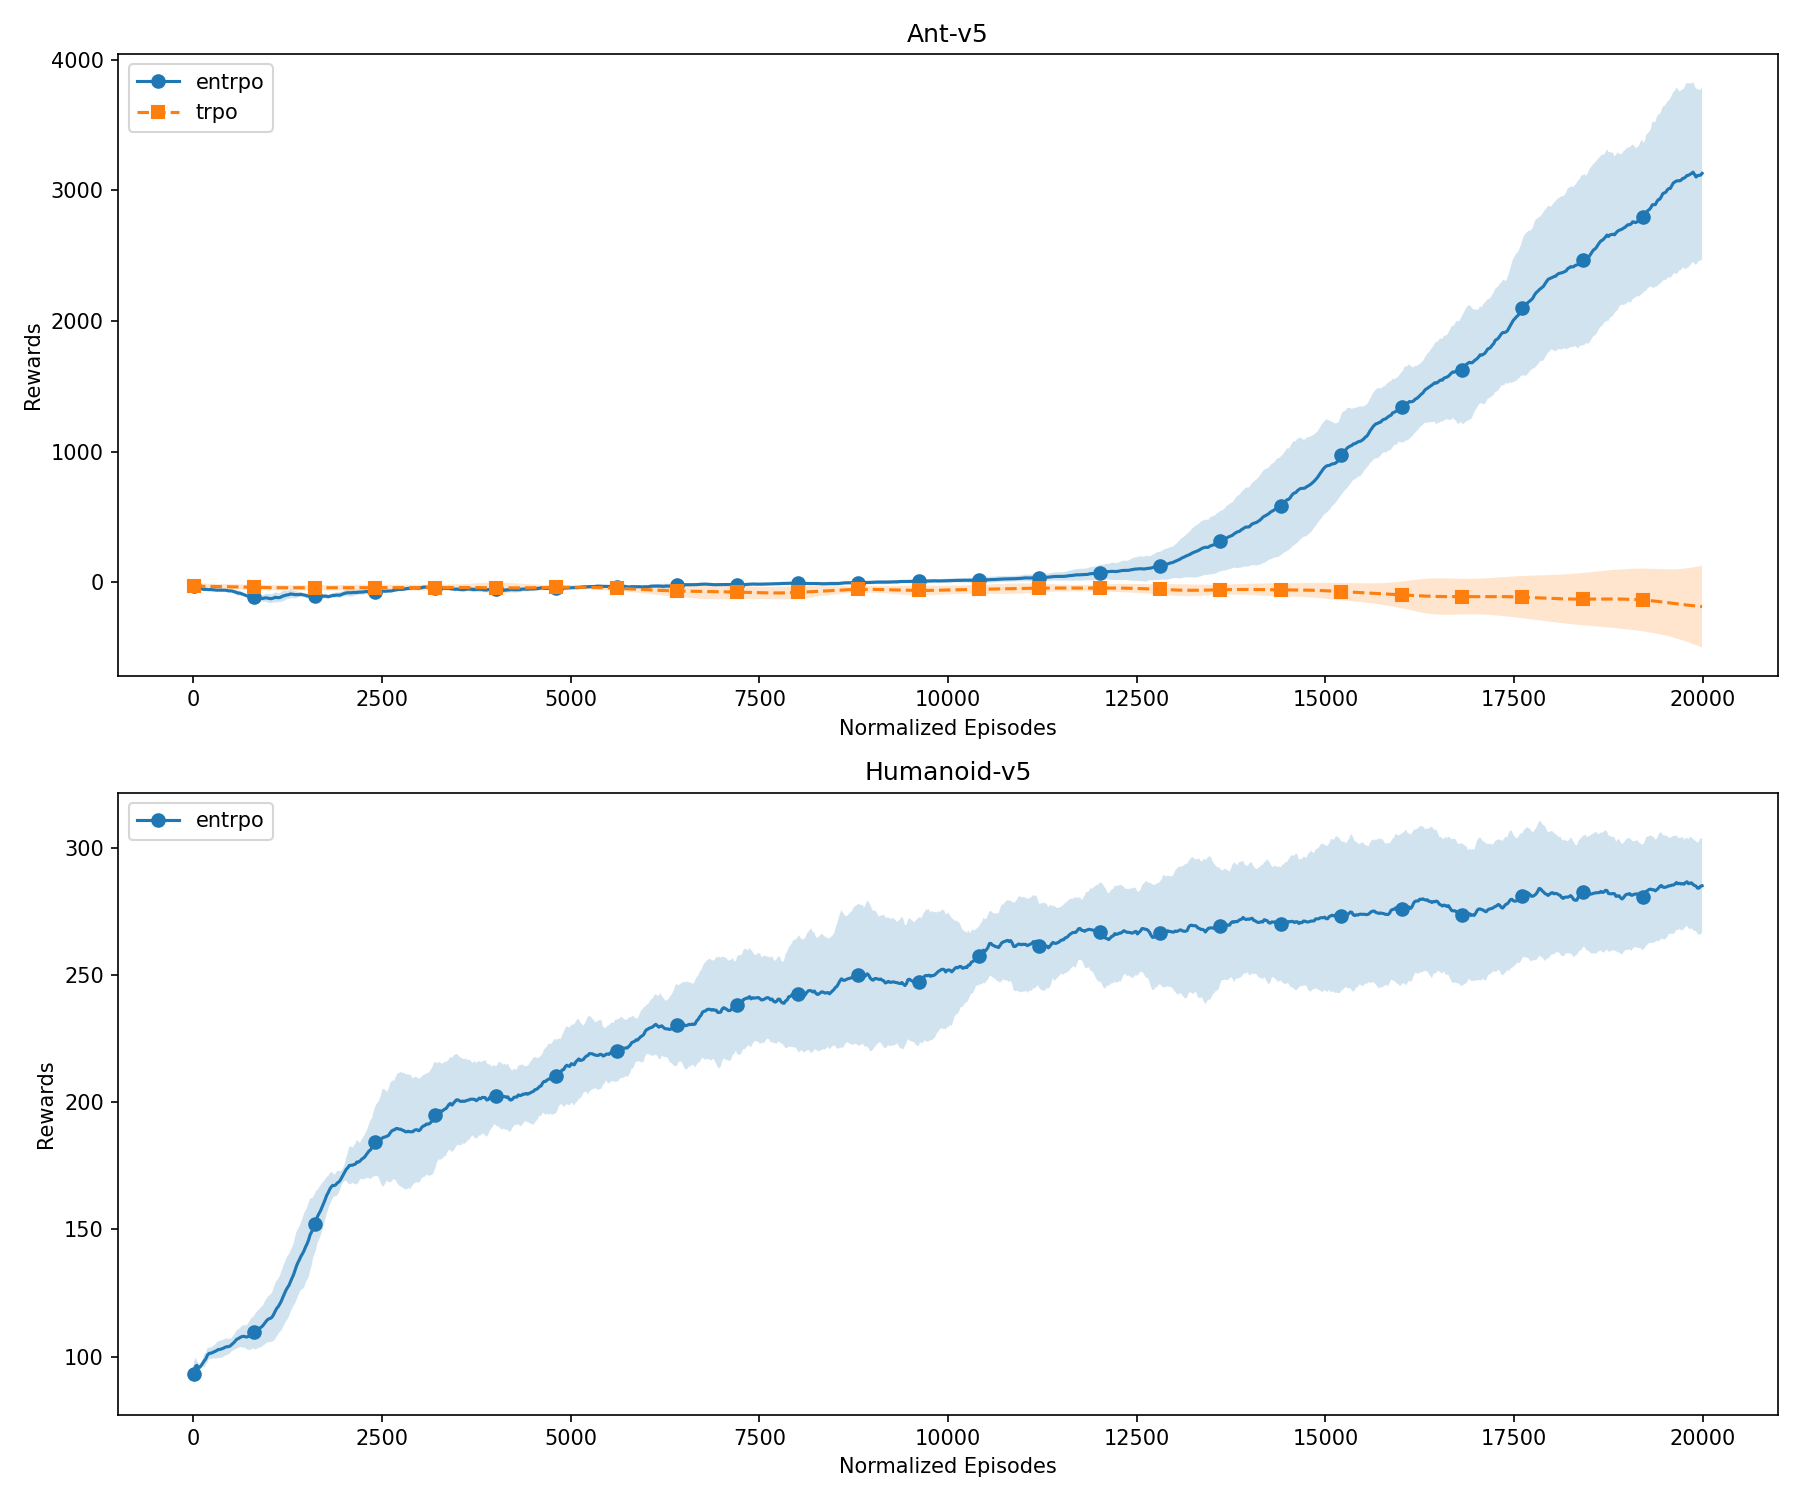
\includegraphics[width=0.8\textwidth]{.assets/resampled_outlier.png}
    \caption{Resampled Rewards with Outlier Removal}
\end{figure}

This plot visualizes the reward distributions after applying smoothing and outlier removal techniques. The presence of large spikes or dips in rewards can indicate unstable learning or catastrophic forgetting. Cleaning the data helps highlight true performance trends and removes misleading fluctuations.

\subsection*{Raw Data}
\begin{figure}[H]
    \centering
    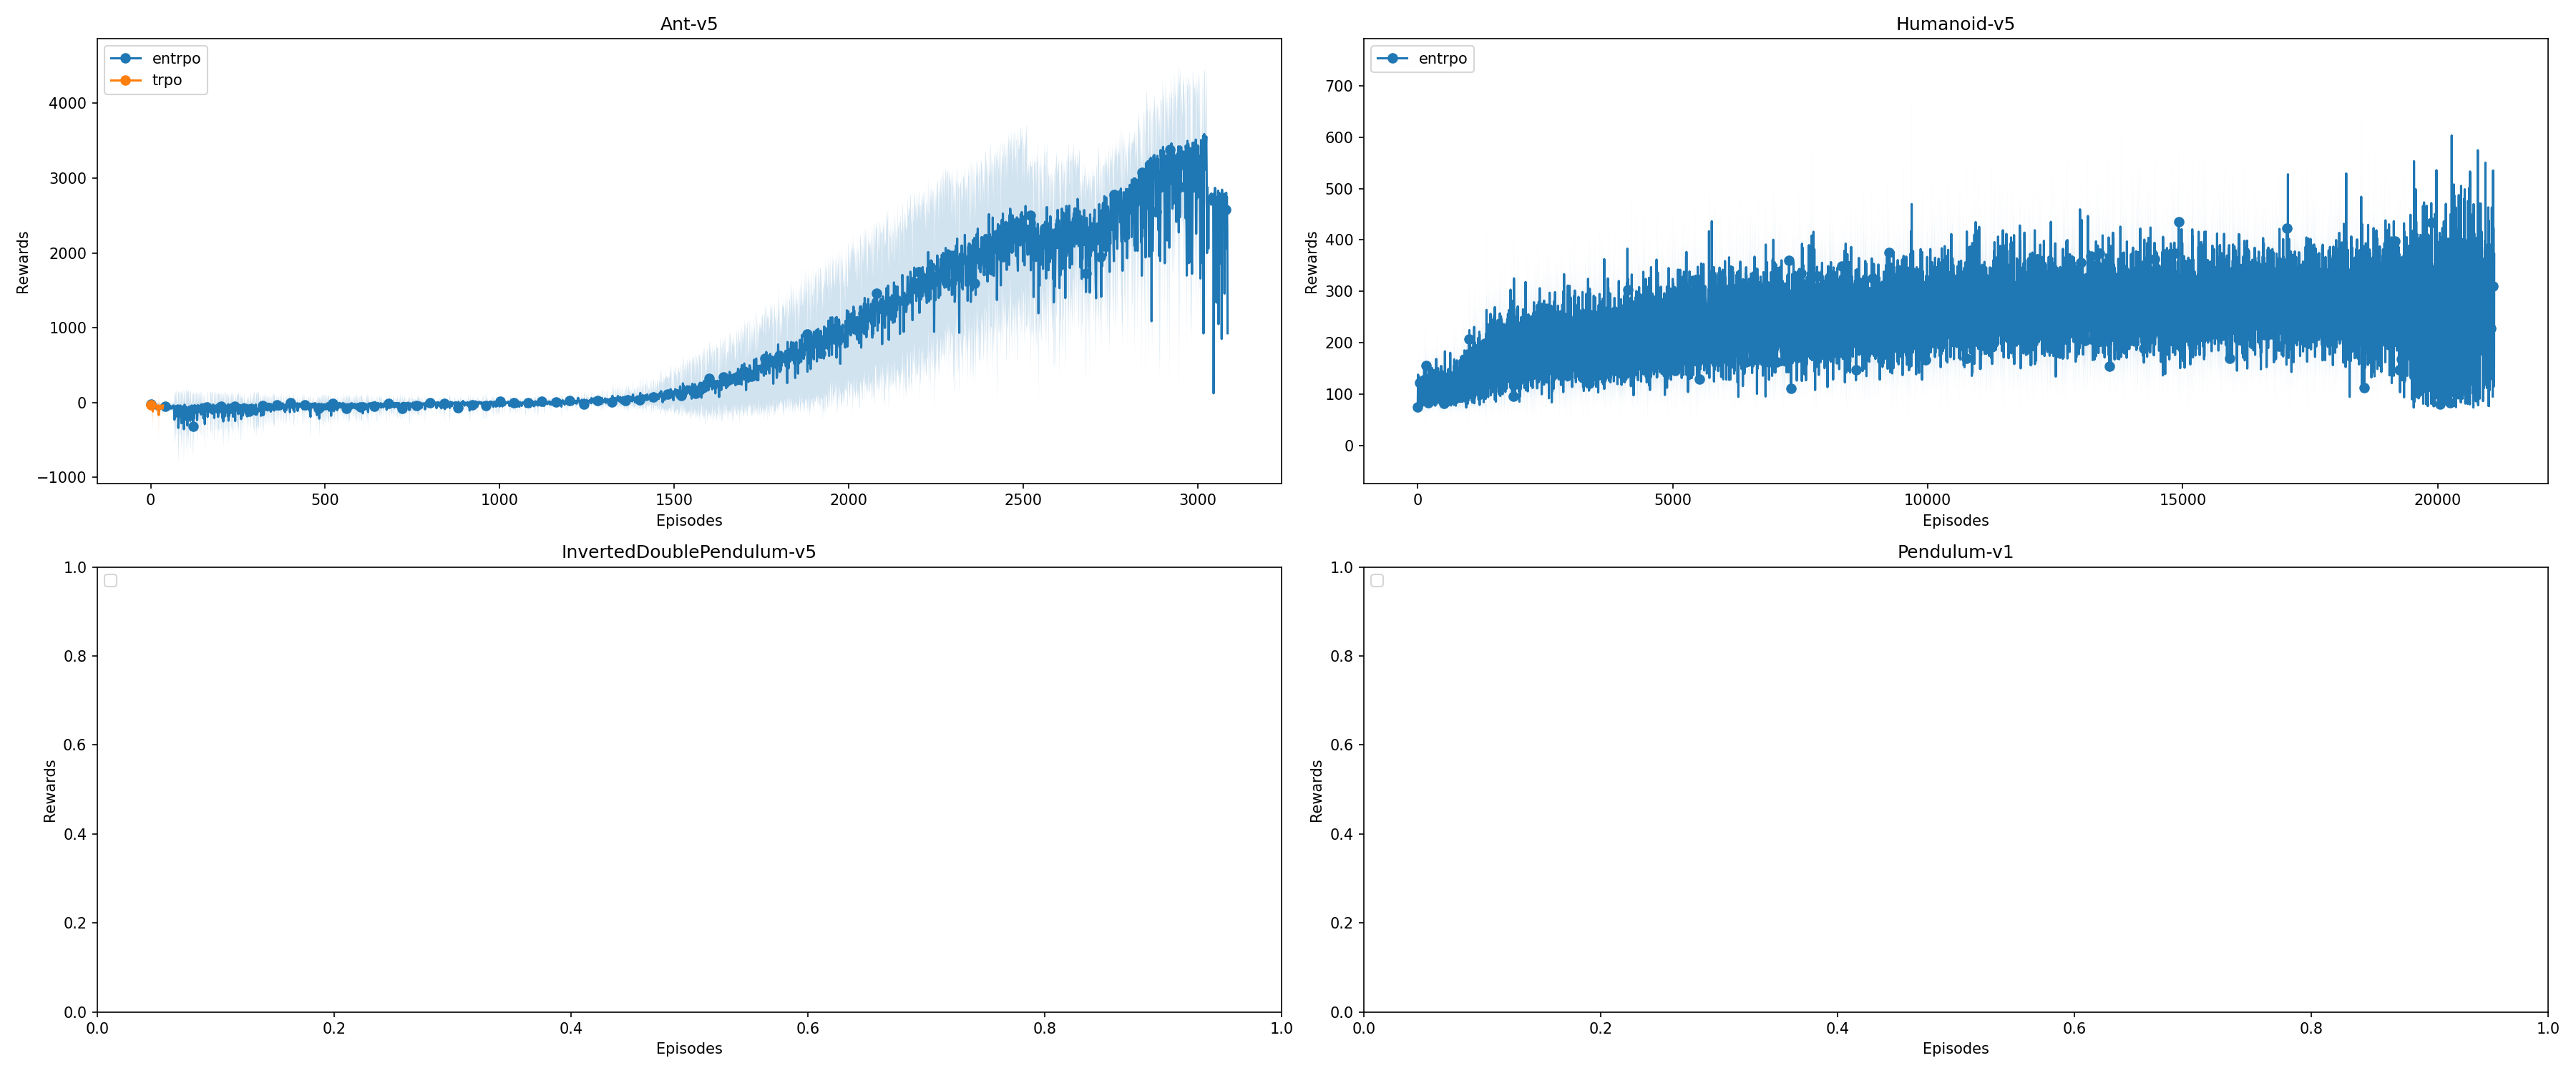
\includegraphics[width=0.8\textwidth]{.assets/raw_data.png}
    \caption{Raw Reward Data for Different Models}
\end{figure}

Since the plots apply resampling and smoothing to compare the models on the same episode scale and make the plots less noisy with data points distribution, the raw data plot shows the actual reward values recorded during training. We can observe that the trajectories will less episodes consumed more timesteps per episodes.

\end{document}
 